\chapter{Evolution de l'interdiction du \riba et Gharar}


a. Un dossier sur un thème lié au cours A partir de trois articles universitaires minimum. -  Introduction : intérêt du thème au regard de l’actualité et/ou de vos propres orientations personnelles ; présentation des articles et de leurs auteurs. Présentation du plan de votre travail. - Synthèse (ne pas présenter les articles séparément mais faire une synthèse à partir des différentes thématiques rencontrées) - Contextualisation de ce thème dans l’islam contemporain, éclairage par le contenu du cours (enjeux, dynamiques, etc). 

\section{Introduction}

En tant que membre du jury de l'Institut des Actuaires, j'ai eu à me prononcer sur certains mémoires présentés par des étudiants sur la \textit{finance Islamique} et \textit{l'assurance Takaful}. Ces mémoires ne couvrent pas les présupposés théologiques et commencent généralement par une présentation des interdits de la loi musulmane, comme par exemple ce \href{http://www.ressources-actuarielles.net/EXT/ISFA/1226-02.nsf/0/8c814ff5f2bae57ec1257e1a004407b6/\%24FILE/Memoire_ISFA_Tontines_et_Takaful_Bendimerad_Version_avec_Couverture.pdf}{mémoire d'actuariat} : 
\begin{quote}
     [pour faire face à ses  engagements, l'assureur],peut, par exemple, inclure des actifs obligataires dont les taux de rendement font apparaître des taux d'intérêt. [...] l'interdiction de l'usage du taux d'intérêt, appelé \textit{\riba} en arabe, est l'un des fondements du droit des affaires musulman.
\end{quote}
Dans la même veine, sont généralement définis les autres interdits, comme le \emph{Gharar}, défini dans le même mémoire comme : 
\begin{quote}
    Le contrat d'assurance peut constituer une perte disproportionnée en faveur de l'un des participants aux dépens de l'autre. Ce caractère d'incertitude, appelé \textit{Gharar} en arabe, est un caractère prohibé par l'Islam surtout lorsque le transfert du risque vers un tiers est total, ce qui est notamment le cas pour l'assureur qui porte entièrement la charge du risque cédé par l'assuré.
\end{quote}
Les mémoires d'actuariat consultés essayent de dépasser ces interdictions, qui soulignent une tension avec les \textit{Hadiths} : 

\begin{quote}
     
A l'issue de l'analyse précédente, l'idée même d'une assurance islamique semble être un contresens. Pourtant, la religion musulmane encourage l'individu à prendre des mesures pour réduire l'ampleur des désastres qui pourraient l'affecter. D'après un Hadith authentifié, le prophète conseille à un croyant de placer sa confiance en Dieu et d'attacher son chameau plutôt que de se limiter uniquement à placer sa confiance en Dieu en offrant la possibilité au chameau libre de s'échapper. L'Islam ne s'oppose donc pas à l'idée de vouloir minimiser les risques et par conséquent elle ne s'oppose pas à faire usage de la loi des grands nombres. Elle exclut certes la spéculation et l'incertitude ainsi que le taux d'intérêt. En revanche, elle compte parmi ses principes la coopération et l'entre-aide mutuelle ainsi que le partage équitable des risques et des bénéfices. Toutes ces bases ont permis de concevoir un modèle alternatif à celui de l'assurance conventionnelle.
\end{quote}
De cette tension naît des solutions techniquement assez complexes.


Intrigué par cette apparente clarté vis à vis de l'interdiction de l'\textit{intérêt} et de l'\textit{l'incertitude} à la base de l'économie moderne, je me propose d'étudier l'évolution de l'opposition de la \emph{\riba} et \emph{gharar} dans les différents courants de l'Islam contemporain, depuis la pensée d'Abduh jusqu'aux frères musulmans et le salafisme. En particulier, nous essayerons d'identifier la voie médiane, entre des lectures libérales (\riba comme usure) et à l'opposé, des musulmans socialistes (\riba comme profit).

L'interdiction des deux notions n'a pas la même importance économique et la \textit{\riba} a donné lieu à plus de développement. En partant de ces études, j'essayerais néanmoins de transposer ces travaux à l'assurance.
Après avoir regardé  à travers l'étude de ces deux notions comment l'économie moderne, pensée au XVIIIè et XIXè siècle questionne l'Islam, je poserai quelques pistes sur le propre questionnement du Christianisme. Après tout, le prêt à intérêt était aussi interdit au Moyen-äge en Europe (Concile de Tours de 1163). Ces pistes seront en particulier nourries par l'étude de la pensée de Saint Thomas d'Aquin sur les taux d'intérêt et comment ces pistes peuvent nourrir la réflexion de la théologie musulmane (et chrétienne) contemporaine. 
 

%---------------------------------------------------------------------------------------------------------------
\section{Vision dans l'Islam Classique de l'interdiction de \riba}

\subsection{une interdiction de la \riba et Gharar}

Pour commencer, il est utile de se référer aux textes à l'origine de ces interdits.
\paragraph{Versets du Coran et Hadiths interdisant la \riba}
Le verset 130 de la Sourate 3, Al-Imran mentionne : 
\vocalize % switch diacritics for short vowels on
\transtrue % display the transliteration
\arabtrue % print arabic text (on by default)
\begin{quote}
 
\TArabe{
 يَا أَيُّهَا الَّذِينَ آمَنُوا لَا تَأْكُلُوا الرِّبَا أَضْعَافًا مُّضَاعَفَةً وَاتَّقُوا اللَّهَ لَعَلَّكُمْ تُفْلِحُونَ
  } 
   [3,125] O vous qui croyez !, ne vivez pas de la \textit{\riba} [produisant le] double deux fois ! Soyez pieux envers Allah ! Peut-être serez-vous bienheureux. 

\end{quote}
\begin{quote}
\TArabe{278
 يَا أَيُّهَا الَّذِينَ آمَنُوا اتَّقُوا اللَّهَ وَذَرُوا مَا بَقِيَ مِنَ الرِّبَا إِن كُنتُم مُّؤْمِنِينَ
279 فَإِن لَّمْ تَفْعَلُوا فَأْذَنُوا بِحَرْبٍ مِّنَ اللَّهِ وَرَسُولِهِ وَإِن تُبْتُمْ فَلَكُمْ رُءُوسُ أَمْوَالِكُمْ لَا تَظْلِمُونَ وَلَا تُظْلَمُونَ
} 
 [2, 278] O vous qui croyez !, soyez pieux envers Allah ! Faites abandon de ce qui [vous] reste [à toucher provenant] de la \textit{\riba}, si vous êtes croyants !
[2, 279] Si vous ne le faites point, attendez-vous à une guerre de la part d’Allah et de Son Apôtre ! si vous vous repentez, alors vous récolterez votre capital sans infliger ou être victime d’une injustice. \sn{Traduction de Blachière, sauf la dernière phrase \cite{ElGamal:BanqueFinanceIslamique}}

\end{quote}

De même, un hadith de Abu Hurayra met au même niveau la \textit{\riba} et le meurtre : 
\begin{quote}
    "Evitez les sept turpitudes !"

- "Quelles sont-elles, ô Envoyé d'Allah?", demandèrent les fidèles.


- "Ce sont, répondit-il :

 

-le polythéisme,

-la magie,

-le meurtre qu'Allah a interdit sauf à bon droit

-l'usurpation des biens de l'orphelin,

-la \textit{\riba},

-la fuite du front au jour du djihad et

-la fausse accusation (de fornication) des femmes vertueuses, chastes et croyantes".
\end{quote}
 
  Nous avons évité à ce stade de traduire le terme de \textit{\riba}, par \textit{usure} ou \textit{intérêt}. Le Hadith rapport par at-Tirmidhî a été utilisé pour appliquer le sens d'intérêt à la \textit{\riba}  : 
 \begin{quote}
     Vendez de l'or contre de l'argent (les quantités échangées étant) comme vous voulez, à condition que ce soit main à main. Vendez du blé contre des dattes sèches (les quantités échangées étant) comme vous voulez, à condition que ce soit main à main. Vendez de l'orge contre des dattes sèches (les quantités échangées étant) comme vous voulez, à condition que ce soit main à main (n° 1240)
 \end{quote}  
 On peut effectivement y lire le refus de l'intérêt mais d'autres lectures sont possibles, en particulier en relevant l'insistance du hadith à une transaction \textit{main à main}, qui permet une transaction claire. Par ailleurs, la valeur du temps n'est pas explicitement mentionnée.
 

 
\subsection{un nouveau contexte avec la naissance du Capitalisme}
Du point de vue du prêteur, le prêt à un prix du fait du risque  que l'emprunteur repaye le prêt, la valeur temps (qui correspond à l'inflation et à la perte d'opportunité d'un investissement aujourd'hui qui rapporte plus plus tard). La pertinence économique de l'intérêt et de la prise de risque est donc justifiée même si cela ne veut pas dire qu'elle l'est d'un point de vue religieux.
Avec l'accumulation des richesses dans les villes italiennes au moyen-âge naît le capitalisme et la finance : comment financer et assurer les bateaux partant de Gênes et remplis de richesse ? Cette irruption de la finance pose de nouvelles questions.  Face à cette accumulation, une réponse théologique chrétienne sera la création de l'ordre mineur par Saint François d'Assise. Et, nous reviendrons sur ses développements, la réflexion de l'université de Paris et de Saint Thomas d'Aquin sur la notion d'usure et de juste prix.  
Ces innovations touchèrent tardivement le monde musulman, au XIXème, avec l'arrivée simultanée de l'industrialisation, qui nécessite des capitaux importants et les débuts de la colonisation. Par l'industrialisation, la capacité productive est fortement augmentée par l'investissement, mais aussi la concentration des risques qui ne peuvent être portée par la solidarité traditionnelle.
Face à cette nouvelle question, quelles sont les réponses proposées par les théologiens musulmans depuis l'arrivée de cette question ?


%---------------------------------------------------------------------------------------------------------------
\section{Elements théologiques apportés}

\subsection{Premières réponses face à la nécessité du prêt}
\paragraph{Le développement du \riba et de l'assurance par les Occidentaux} Les prêts à intérêt ont toujours existé au sein de l'Empire Ottoman\cite{Gilbar:Qadi}, et proposés par des familles grecques, arméniennes ou Juives (et en Iran par les arméniens et zoroastriens). A ce premier Groupe, s'ajouta les banques commerciales européennes ou les banques "étrangères-locales" comme la banque impériale ottomane au XIX.
De la même façon pour les assurances, Ibn Abidin, représentant de l'école officielle de droit Hanadi dans l'empire ottoman, suggère le compromis suivant : il est licite d'établir ds contrats d'assurance portant sur les risques encourus à l'intérieur du royaume islamique - le Dar al Islam -à condition que ces contrats soient conclus avec une compagnie d'assurance ayant son siège hors de pays de l'Islam. 

\paragraph{Utilisation de prêt à intérêt par les musulmans malgré l'interdiction du \textit{\riba}.} La \textit{\riba} a pu poser des problèmes dans son implémentation, en particulier pour les grands marchands (tujjār).  
Pour l'école Hanafite, le terme de \riba peut être traduit par usure, dans le sens d'un taux d'intérêt exhorbitant, à l'opposé de l'intérêt raisonnable, le \emph{ribh}. L'autre interprétation dominante, attribuée à 'Abdahallah Ibn 'Abbas, permet d'expliquer la notion du Coran de double capital par la pratique du \textit{\riba al jâhiliyya} (préislamique), avec des taux d'intérêt très élevés avec des intérêts pouvant dépasser le capital en cas de non-paiement. A l'opposé de ces analyses plus ouvertes, la position de l'école Hanbalite fut l'interdiction pure de l'intérêt. Pour contourner l'interdit du \riba face à la nécessité, les marchands musulmans mirent en place des montages complexes où l'intérêt était déguisé en une \textit{double vente} (\emph{mukhâtra}) avec deux ventes fictives successives permises par la \textit{sha'ia}: 
\begin{itemize}
    \item la première, le préteur vent un objet à l'emprunteur pour une somme équivalente au capital et à l'intérêt. l'emprunteur s'engage à payer la valeur de l'objet à la fin de la période (techniquement, une vente avec paiement différé). 
    \item A la fin de cette première transaction, l'emprunteur revend le même objet pour la valeur du principal (techniquement, une vente à terme).
\end{itemize}
 Cependant, l'étude des jugements des cours religieuses au moyen-orient entre le XVI et le XVIII montre que malgré ces montages, des exemptions partielles ou totales de paiement de l'intérêt du fait de son incompatibilité avec l'Islam \sn{GILBAR, GAD G. “The Qadi, the Big Merchant and Forbidden Interst (Ribā).” British Journal of Middle Eastern Studies, vol. 39, no. 1, 2012, pp. 115–36, http://www.jstor.org/stable/23264404. Accessed 3 May 2022.}
 

\section{la pensée d'Abduh et Rida}
\subsection{position d'Abduh} Le Cheikh {Muhammad Abduh} (1849 - 1905) Egyptien, successeur d'Al Afghani, est la figure marquante du réformisme islamique. Il s'oppose au colonialisme atteignant alors l'Egypte. Son séjour  parisien le convainc de la nécessité de réforme de l'Islam et l'initie aux réflexions intellectuelles occidentales et en particulier François Guizot. A sa suite, il il pense l'Islam comme civilisation et pas uniquement comme Religion, avec la notion de progrès lié à la civilisation. Il n'y a pas d'opposition pour lui entre Foi et Raison, la religion musulmane étant \textit{raisonnable}.    Dans son livre \citet{Abdou:Rissalat}, il part de la Raison pour montrer le besoin que l'homme ne se fixe pas sa propre loi.

Il montre tout d'abord la naissance des besoins et des liens entre les hommes. Idéalement ces liens seraient ceux de l'amour : 
\begin{quote}
    Nul ne met en doute que chaque membre d'une société a besoin
des autres membres; et chaque fois que l'individu accroître ses exigences
dans la vie il ressent plus fortement le besoin de recourir au concours
de ses semblables. Ainsi se développent les besoins et à leur suite s'étendent
les relations de la famille à la tribu, de celle-ci à la nation, et finalement
au genre humain tout entier, comme le montre notre époque . Ces
besoins qui créent dans le sein de chaque nation (surtout dans le sein de
celles qui méritent vraiment ce nom) des relations et des rapports
spéciaux la distinguant des autres nations, sont le besoin de se procurer
sa subsistance, celui de profiter des biens de la vie, celui d' acquérir
les choses désirables et d'éloigner de soi celles qui déplaisent. 
Si la vie de l'homme se déroulait selon les lois de la nature, telles
que nous les voyons appliquées aux autres êtres vivants, les besoins
que nous venons de citer auraient été parmi les facteurs les plus puissants
de l'amour entre les individus[...].  

[\ldots]
Si par contre, l'intérêt se mêle aux relations amicales, et si chacun des amis exige un prix pour son amour, celui-ce se change en esprit d'exploitation, il se reporte sur l'effet utilitaire et se transforme chez l'un des amis en un abus de la force, et chez l'autre, en peur avilissante, en dissimulation et en hypocrisie.
\cite[p.66]{Abdou:Rissalat}
\end{quote}
Mais l'homme ne vient pas selon les lois de la nature car il est inconstant : 
\begin{quote}
 l 'homme
a été créé avec un caractère inconstant; quand le malheur l'atteint
il est abattu, et quand il acquiert quelque bien il devient insolent.
(C. ch. 70, v. 19 à 21). [...]
Chaque fois que la mémoire et l'imagination les poussent à
éviter quelque chose qui leur inspire de la crainte ou à atteindre un
objet qui leur fait envie, leur intelligence leur ouvre une porte de la
ruse ou leur découvre une voie de la violence ; alors le rapt remplace
l'échange pacifique, la dispute prend la place de l'union et la conduite
de l'homme riche s 'appuie plus que sur l'astuce et la violence.
\cite[p 68]{Abdou:Rissalat}
\end{quote}
il montre qu'on peut accéder à l'équité par des voies naturelles mais qu'à la foi pour les masses et pour éviter la corruption des élites, il est nécessaire de s'appuyer sur loi externe.
\begin{quote}
[...] ] le genre humain
a surtout besoin, pour conserver son existence, de l'amour ou d'un
sentiment qui le remplace.
A différentes époques il y a eu des penseurs qui ont fait appel à
l'équité ; ils ont pensé, et même quelques mystiques ont exprimé cette
pensée par de nobles paroles, que l'équité remplace l'amour. Cette
assertion ne manque pas de sagesse, mais qui est-ce qui peut établir les
règles de l'équité et amener la totalité des hommes à se soumettre ?
\cite[p 69]{Abdou:Rissalat}
\end{quote}

Suivre la Loi de Dieu, ordonner le bien est alors supérieur à la foi : 

\begin{quote}
  le Coran indique
qu'il n'y a pas de condition meilleure que celle des hommes qui ordonnent
le bien et défendent le mal: \begin{quote}
    Vous êtes les meilleurs parmi les hommes,
vous ordonnez le bien, vous défendez le mal et vous croyez en Dieu. (Cor. ch. 3, v. 106.) 
\end{quote} 
 
Dans ce verset le fait d'ordonner le bien et de
défendre le mal est mentionné avant la foi en Dieu, bien que la foi soit la base même sur laquelle s'appuient les bonnes oeuvres. 
\cite[p 121]{Abdou:Rissalat}
\end{quote}

\paragraph{Conséquence pratique pour la \riba}
'Abduh liste alors une liste de maux que l'Islam permet d'éviter : 
\begin{quote}

[l'Islam] nous invite par dessus tout à dépenser notre bien pour les oeuvres
charitables et souvent il en fait l'expression de la foi et la manifestation
d'une bonne conduite; il déracina par là, du coeur des pauvres, la rancune
et la haine contre ceux que Dieu a favorisé des biens terrestres ; il leur
inspira l'amour pour les riches, tout comme il fît naître dans le coeur de
ceux-ci la pitié pour les malheureux ; ainsi il développa la confiance dans
le coeur de tous les hommes. Quel remède plus efficace contre les maux
dont souffre la société: « C'est une faveur que Dieu accorde à qui il veut,
car Dieu est d'une bienfaisance sans bornes. » (Cor. ch. 57, v. 21.)
\textbf{L' Islam a fermé les deux portes du mal, il a bouché les deux sources
qui minent l'intelligence et détruisent la richesse, en frappant les boissons
enivrantes, les Jeux de hasard et l'usure, d'une interdiction absolue qui
n'admet pas d'infraction.}
\cite[p 122]{Abdou:Rissalat}
\end{quote}
Ainsi, parmi ces maux figure la \riba traduit ici par \textit{usure}.

\paragraph{Pratiquement : l'avis d'Abduh sur l'ouverture de la Caisse d'Epargne en Egypte}
L'ouverture de la Caisse d'Epargne et la répugnance d'un certain nombre de musulmans à toucher les intérêts poussèrent la caisse d'épargne à demander à 1903 une Fatwa à Abduh \cite{Jomier:AdbouCaisseEpargne}. Cette fatwa semble n'avoir jamais existé. En revanche, Ce fut à la requête d'un particulier mais en fait pour la
Compagnie d'Assurances sur la vie Gresham. La Compagnie d'Assurances al-Chark,
au Caire,  conservait une copie d'une fatwa d'Abduh \textit{écrite initialement pour un particulier} afin de la montrer à ses clients, le cas échéant. Le
client effectue des versements réguliers et périodiques par tranches successives
prévues d'avance ; la compagnie les encaisse et se charge de faire fructifier cet
argent. Finalement, à l'échéance, la société remboursera le total des versements
effectués augmenté des bénéfices résultant de la fructification. La fatwa admet
la licéité d'une telle opération en des termes qui, au fond, s'appliqueraient à toute
société en commandite. Il faut noter que la revue Al-Manâr de \textit{Rashid Rida} ne nia pas l'authenticité de cette fatwa après la mort d'Abduh mais protesta contre l'extension faite à toute assurance vie.

\paragraph{la note de la revue Al-Manâr de 1903}


Face aux scrupules de 3000 musulmans à toucher les intérêts (fa'ida), un échange eu lieu entre le directeur de la Caise d'Epargne et Abduh, échange repris par la revue \textit{Al-Manâr}. Abduh y maintenait fermement le principe de
l'interdiction absolue de l'usure (al-ribâ) ; mais il ne classait pas le cas de la Caisse
d'Epargne avec ceux de l'usure. Il l'assimilait à celui d'une société en commandite
(chirkat al-mod'âraba). A la suite de cette discussion, la loi fut modifiée en 1904 : 
 

\begin{quote}
 Il est prévu dans l'article premier que le client devra signer un
formulaire imprimé dans lequel il déclarera donner au Directeur Général de la
Poste tout pouvoir pour faire fructifier les sommes déposées, d'une façon licite et
en excluant toute opération usuraire. Il déclare permettre au Directeur de la Poste
de joindre ses dépôts à ceux des autres clients pour les faire fructifier en commun
à condition de recevoir une part de bénéfices (al-ribh') proportionnelle à ses
versements. On notera que dans cet article comme dans tout le reste de la loi le
mot de \textit{fâ'ida}, intérêt, est totalement absent. \cite{Jomier:AdbouCaisseEpargne}
\end{quote}

\begin{quote}
    L'article deux stipule entre autres ce qui suit. Il évite de parler de tant pour
cent, formule qui rappelle trop les intérêts. Il note que la part des bénéfices ne
dépassera pas un pour quarante du capital et le surplus, s'il y en a, reviendra à
l'administration postale à titre de compensation pour les services rendus et les
frais que ceux-ci comportent. L'assimilation à la société en commandite est ainsi
mise en accord avec le fait que la proportion des bénéfices touchés est fixe. On
notera que la proportion de un pour quarante est familière aux oreilles des
musulmans pieux puisque dans un certain nombre de cas le montant de la Zakat
atteint ce chiffre.
\end{quote}


Abduh développe la raison de cette position dans la fatwa et la note du manâr du 18 mars 1904: 
\begin{quote}
    La raison de l'interdiction de l'usure est de faire cesser l'injustice et de conserver les vertus de solidarité et de bonté mutuelle
\end{quote}
On voit donc la position d'Abduh comme ferme dans les principes et ouvert dans l'application pour vivre de l'Esprit pourrait-on dire, même si cela se traduit par une subtilité juridique.


% - ----------------------------------------
\subsection{L'approche de Rashid Rida sur la \riba} 

Rida est l'un des successeurs spirituels de Abduh. Il fonda avec Abduh la revue néo-réformiste al-Manâr en   1898. Elle définit sa politique éditoriale à l’égard « de la civilisation occidentale » sous forme de deux impératifs : 
\begin{quote}
    \item  1/ Il faut que la terre musulmane puisse rattraper l’Europe sur le plan des sciences modernes, de l’industrie et de l’innovation technique. 
    \textbf{ }2/ En contrepartie, il faut déclarer une guerre sans merci à tout ce qui a accompagné l’entrée des Européens en terre musulmane comme décadence morale et mauvaises mœurs
\end{quote}

\paragraph{Une lecture de la \riba originale à la base de l'économie Islamique } Si la position de Rida vis à vis de la liceité de l'intérêt est dans les faits la même que celle d'Abduh, Rida pose son raisonnement par une analyse détaillée des versets du Coran et des Hadiths parlant de \riba  \cite{Siddique:DemystifyingRiba}. 
Rida part de l'analyse du mot \riba comme \textit{excès}, et en particulier reprend l'analyse de Co 3,125 présentée au début d'un excès lié à la renégociation de la dette. De là, il conclut que ce qui est interdit par le Coran sont les intérêts ajoutés à la fin de la période de prêt (\riba ’l-jahiliyyah). D'une certaine façon, ce sont les intérêts composés ("intérêt d'intérêt") qui sont interdits, ce qui arrive en cas de non paiement à la fin de la période définie. Cette distinction permet à Rida d'autoriser les intérêts bancaires :
\begin{itemize}
    \item ils ne doublent pas les taux
    \item l'ajout d'un intérêt fait partie du principal de la même façon que le prix d'une vente à crédit (\emph{\riba al-buyu}) qui ne sépare pas principal et intérêt et qui est autorisé par le Coran.
\end{itemize}

 La distinction de Rida entre la \riba interdite dans le Coran et celle des Hadiths est présentée dans le graphique \ref{fig:MinorityRiba}.

 \begin{figure}[h!]
     \centering
     \sidecaption{\cite{Siddique:DemystifyingRiba}, une séparation entre Coran et Hadith}
      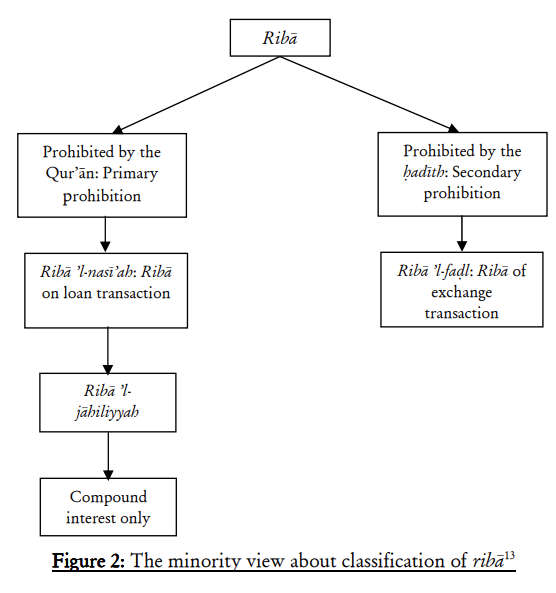
\includegraphics[width=0.6\textwidth]{CourantsIslamContemporain/ImagesCourantsIslamContemporain/RibaRida.png}
      \caption{La présentation du Riba selon Rida, dite minoritaire}
     \label{fig:MinorityRiba}
 \end{figure}
 Cette distinction entre \riba du Coran et \riba du Hadith permettait à Rida de légitimer la notion d'intérêt. Il ne sera cependant pas suivi sur ce point par la majorité des jurisconsultes qui étendront l'interdiction de la \riba du Coran à tout intérêt, simple ou composé (intérêt d'intérêt). En revanche, ces derniers adopteront sa distinction entre les différents \riba du Coran et du Hadith. Mais cette distinction, loin de simplifier le sujet, rend les discussion assez techniques, en particulier parce que les différentes écoles appliquent aux hadiths des méthodes d'analyse différentes que celles appliquées sur le Coran. 
 

 
\paragraph{Les frères musulmans} L'exemple de la \riba montre la capacité d'adaptation d'Al Banna, le fondateur des frères musulmans.
La \riba est interdite dans le programme des frères musulmans, comprise dans le sens large et interdisant le taux d'intérêt (ou en incitant à ne pas l'utiliser) : 
\begin{quote}
    III. 2 interdiction de pratiquer l'usure, orienter les banques vers cette interdiction, le gouvernement doit donner l'exemple en abandonnant l'\textit{intérêt} fixé par les banque du prêt et du prêt industriel, etc. \textit{programme des frères Musulmans, 1936}
\end{quote}

Cependant, al-Banna, avait admis la licéité des sociétés en commandite qui verse des dividendes et les Frères avaient, peu avant 1948, fondé quelques ateliers
ou sociétés financées par ce procédé, contournant ainsi le besoin d'utiliser le mot fâ'ida, intérêt.


\paragraph{les nouveaux penseurs}  Nous avons cité Muhammad Zahid Siddique
\cite{Siddique:DemystifyingRiba}, professeur pakistanais d'économie, qui nous semble un bon exemple des réformistes du droit, qui se situe dans une logique de l'adaptation du \emph{figh} aux nouvelles problématiques. En 


, par l'inclusion de nouvelles techniques, ici historique et économique. Tout d'abord, il montre montre que la distinction de Rida entre la \riba du Coran et la \riba du Hadith est basée sur une argumentation circulaire. Il essaye de donner du sens à l'approche classique juridique tout en essayant de la simplifier et l'homogeniser, pour qu'elle soit applicable. Il déduit 5 implications : 

\begin{quote}
    \item illeicité d'un marché de prêt. Néanmoins les prêt sont possibles si ce sont des actes d'entraide, en particulier au sein d'une famille.
    \
    
\end{quote}
Enfin, il travaille sur la distinction entre \emph{Bay} (vente, souvent à crédit) et \riba, en prenant au sérieux l'objection des incroyants "vraiment, la vente (à crédit) \emph{bay}, c'est la même chose que la \riba "
.  essaye de réduire les  Puis, il applique Des discussions casuistes, on peut 
L'approche de Rida de séparation des \riba du Coran et des Hadiths a été remis en cause par une approche des textes \cite{Siddique:DemystifyingRiba}
Des discussions casuistes, on peut 
 \begin{figure}[h!]
     \centering
     \sidecaption{\cite{Siddique:DemystifyingRiba}, le Hadith expliquant le Coran}
      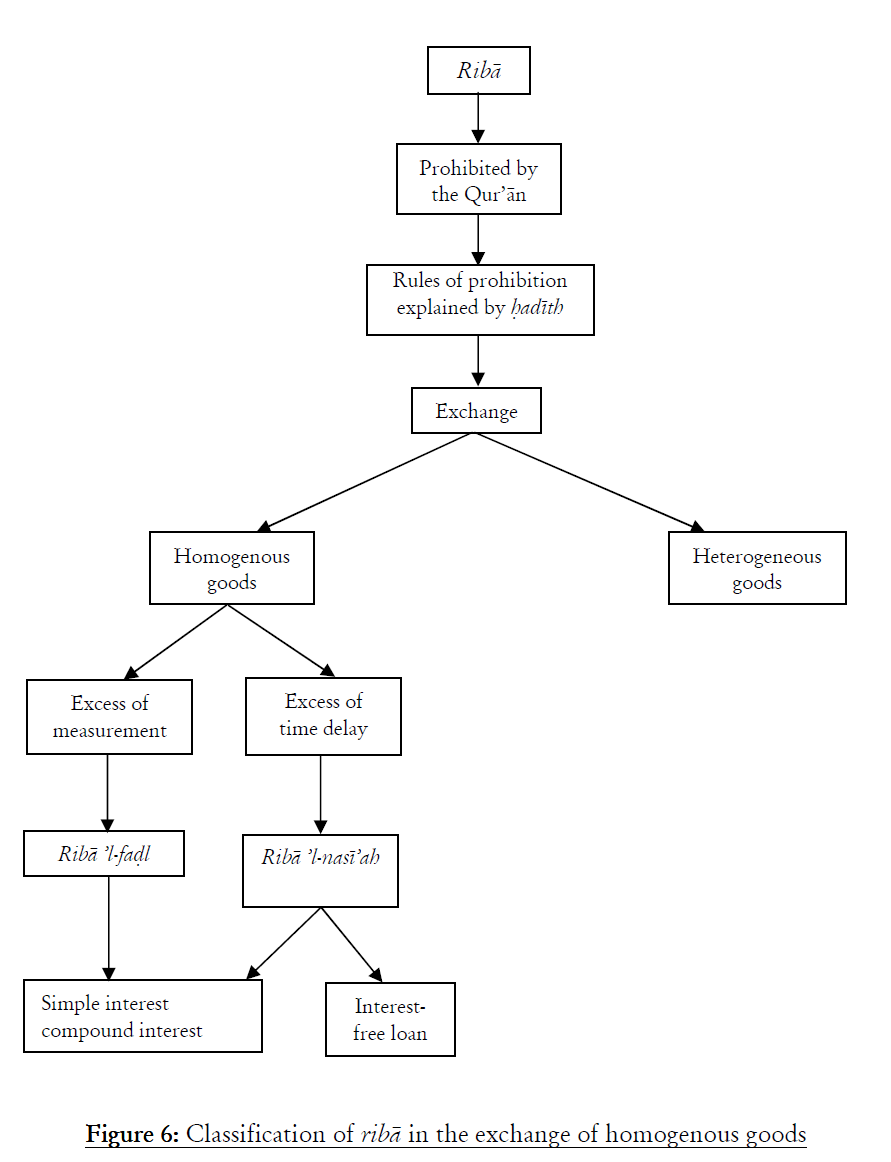
\includegraphics[width=0.6\textwidth]{CourantsIslamContemporain/ImagesCourantsIslamContemporain/RibahomogeneousGoods}
      \caption{La présentation du Riba selon \cite{Siddique:DemystifyingRiba}}
     \label{fig:MinorityRiba}
 \end{figure}
 

%---------------------------------------------------------------------------------------------------------------
\section{Naissance de la finance et de l'assurance Islamique}

\subsection{Ce que l'on voit : Malaisie,...} 

\paragraph{une pratique supposant une \textit{shari'ah} qu'on ne peut interroger}

\subsection{Quelle est la théologie sous-jacente}

\paragraph{Une évolution de la shari'a par les principes} Mohammed Talbi 
\begin{quote}
    Il existe
trois principes en islam permettant de faire évoluer le droit et de
l'adapter
à la réalité, 

la \emph{maslaha} c'est-à-dire l'utilité publique, un
concept qui date du II\textsuperscript{e} siècle de l'hégire, 

la
\emph{zharoura}, la nécessité, c'est un principe fort puisqu'il est dit
que "la nécessité rend permis l'interdit" ; 

et les \emph{maqassid}, les
finalités de la loi. 

\begin{Synthesis}
On part des principes contre les principes. 
\end{Synthesis}
\sn{voir p. \pageref{TroisPrincipesEvolutionsShari}}
\end{quote}


\section{Conclusion}

\paragraph{une variété importante de vision mais toujours basée sur la sharia}

\paragraph{une réflexion sur la base de la Sharia'}
voir ce que Candiard dit de ce théologien qui dit de ne pas faire de Kalam mais du droit.

\paragraph{quel pourrait être les pistes de Kalam, quelques pistes de l'expérience occidentale ?}

\paragraph{St Thomas et l'usure : une réflexion autonome de la théologie}

\paragraph{extension du juste prix dans les risques : la dimension actuarielle}
\paragraph{Au XIXème, réflexion neo-thomiste et patristique pour sortir du carcan}
Après avoir regardé comment l'économie moderne, pensée au XVIIIème et XIXème questionne l'Islam à travers l'étude des différents courants de l'Islam contemporain, je poserai quelques pistes sur le propre questionnement du Christianisme. Après tout, le prêt à intérêt était aussi interdit au Moyen-äge en Europe. Ces pistes seront en particulier nourrie par l'étude de la pensée de Saint Thomas d'Aquin sur les taux d'intérêt et comment ces pistes peuvent nourrir la réflexion de la théologie musulmane. 

Nous catholiques au XIX par rapport à la modernité: renouveau thomiste et patristique. Liberté de pensée par rapport aux questions de l’époque
« A quoi on tient en vrai »
Le raccourci de certains théologiens musulmans : faire le court circuit pour repenser les choses : obsession juridique. Comment on sort du droit ? En faisant de la théologie. Et pour cela retour à la tradition
Voile
Le coran la dit donc il faut se voiler. Voile : hijab n’est pas dans le coran. Rideau
Zina : qu’il faut cacher
Jilbab pour les filles et femmes du prophète 
Ibn el jahouzi : voile non mentionné. Dimension non religieuse

Des écrits au XX. Deux raisons : les femmes vont occuper plus de rôle dans l’espace publique.
Et renouveau de l’anti théologie. Le voile est une question de théologie. Question de la foi
	⁃	Saint Paul : la foi et les œuvres
	⁃	On comprend croyant non pratiquant
	